\chapter{Fission yields for r-process nuclei}\label{chap:rprocess}

\section{The role of fission in the astrophysical r process}
One of the outstanding mysteries in astrophysics is the origin of heavy elements. It is thought that heavy elements are formed in violent, neutron-rich astrophysical environments, such as core-collapse supernovae or neutron star mergers, as the result of a rapid neutron capture process. This process, generally shortened to ``r process'', involves bombardment of small seed nuclei with neutrons followed by beta decay toward the valley of stability.  This process is illustrated schematically in Figure~\ref{fig:rprocpath}.

\begin{figure}
	\centering
	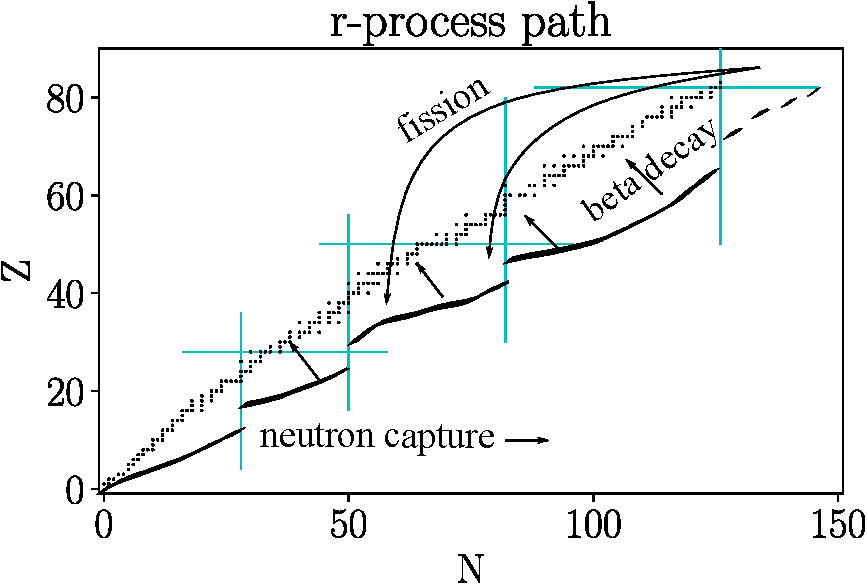
\includegraphics[width=0.8\linewidth]{TeX_files/rProc_path}
	\caption[Schematic overview of the r process. The competition between neutron capture and beta decay increases the mass of a seed nucleus until it reaches the region where fission dominates (spontaneous, beta-delayed, or neutron-induced).]{Schematic overview of the r process. The competition between neutron capture and beta decay increases the mass of a seed nucleus until it reaches the region where fission dominates (spontaneous, beta-delayed, or neutron-induced).}
	\label{fig:rprocpath}
\end{figure}

Fission plays an important role in the r process. The competition between neutron capture and beta decay determines the manner in which the r process proceeds. Fission places an upper limit on the mass of isotopes that can be produced in an r-process scenario, as fission lifetimes for heavy and superheavy isotopes become small enough to compete with neutron capture and beta decay for very heavy systems. Also, as will be discussed shortly, fission fragments of isotopes in this mass region are thought to shape the rare earth peak around $A\approx165$.

Elemental abundance patterns in some old, metal-poor stars outside our solar system have been found to resemble that of our own~\cite{Arnould2007}, and it has been suggested that fission may be responsible for this ``universal r process'' via a mechanism called fission cycling~\cite{Beun2008}. Once a heavy nucleus fissions, its fragments can then absorb more neutrons and make their way back up the r-process chain. In a neutron star merger environment, the system may undergo somewhere between 1-4 fission cycles before settling into its final state~\cite{Mendoza2015}.

In order to guide experimental and theoretical efforts and to reduce uncertainties in the abundance pattern, sensitivity studies (in which model inputs are tweaked to measure their effect on the final yield) can estimate the impact of a particular set of observables, such as fission fragment yields, on the r-process abundance pattern. Sensitivity studies indicate that fission yields primarily affect the elemental abundances between the second r-process peak ($A\approx130$) and the rare earth peak ($A\approx160$)~\cite{Goriely2015a, Eichler2015}. This can be seen in Figure~\ref{fig:rprocabundances}, in which four different sets of phenomenological fission fragment yields were used to compute abundances. That this region is sensitive to fission yields should come as no great surprise, since most naturally fissile nuclei produce fission fragments in this region.

\begin{figure}
	\centering
	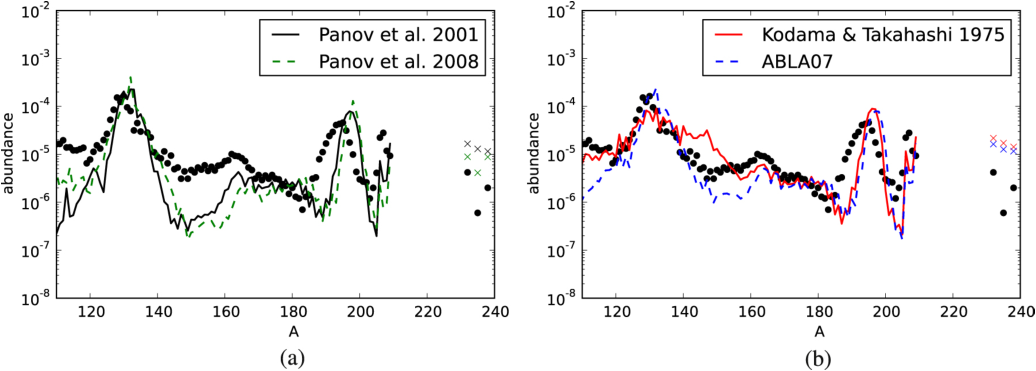
\includegraphics[width=0.9\linewidth]{TeX_files/rProc_abundances}
	\caption[Final abundance patterns from four different simulations of neutron star merger ejecta, each using a different model for the fission fragment yields. The results are presented in two graphs solely for visual clarity. The dots represent the known solar r-process abundance pattern. Figure from~\cite{Eichler2015}.]{Final abundance patterns from four different simulations of neutron star merger ejecta, each using a different model for the fission fragment yields. The results are presented in two graphs solely for visual clarity. The dots represent the known solar r-process abundance pattern. Figure from~\cite{Eichler2015}.}
	\label{fig:rprocabundances}
\end{figure}

R-process network calculations combine nuclear physics inputs, such as decay lifetimes and fission fragment yields, with astrophysical inputs, such as temperature and neutron density, to simulate the complex competition between various nuclear decays. Such calculations require quality inputs from a variety of sources. Many nuclei of interest to the r process are too neutron-rich or too heavy to be studied in a laboratory, which means that theoretical calculations provide essential model inputs. These calculations should be performed using models that are known to extrapolate reliably. As a global microscopic model that is designed to reproduce data across the nuclear chart, nuclear DFT is well-suited for this type of problem.

\section{Fission fragment yields for r-process nuclei}
The predictive power of r-process network calculations could be improved with a global survey of microscopically-calculated fission fragment yields, including yields from spontaneous fission, beta-delayed fission, and neutron-induced fission. However, the computational expense associated with full Langevin calculations makes this method impractical for large-scale survey calculations. Instead, we have developed an efficient model for estimating fragment yields using the nucleon localization function which is designed for large-scale calculations like this. Our model is introduced in Section~\ref{sect:FragID}, with a detailed description in Appendix~\ref{append:Fragments}.

%Something interesting, and perhaps the kind of thing that might fit in with your thesis, is that there is a predicted four-hump pattern for the A=278 isobars in the SPY model (Scission Point Yield)~\cite{Goriely2013}. This doesn't show up in the GEF, so far as I know, but it's interesting to think about. That could be an interesting thing to check a bit more carefully, since such a thing has never been observed experimentally. Also, 278Cf happens to be exactly halfway in between 266Cm and 290Fm. PS they actually show a PES for 278Cf in their Figure 3. I'm not 100\% convinced.

Initial calculations were performed using the isotopes $^{254}$Pu, a neutron-rich isotope of plutonium predicted to have a large fission flow during neutron star mergers~\cite{Vassh2019}, and $^{290}$Fm, an extremely neutron-rich isotope of fermium. For each isotope, a 1D PES was calculated up to the outermost isomer state by constraining $Q_{20}$ and leaving the other degrees of freedom unconstrained. Between the isomer state and the outer turning line, the PES was expanded to include $Q_{30}$ in order to account for mass asymmetry between the fragments. The WKB method was used to estimate relative probabilities along the outer turning line, at which stage fragment pairs were identified using the localization-based method described in Appendix~\ref{append:Fragments}. Sample localizations, along with the resulting PESs and distributions are shown in Figures~\ref{fig:254Pu-yield} and~\ref{fig:290Fm-yield}.

\begin{figure}%
	\centering
	\subfloat[$^{254}$Pu neutron localization]{{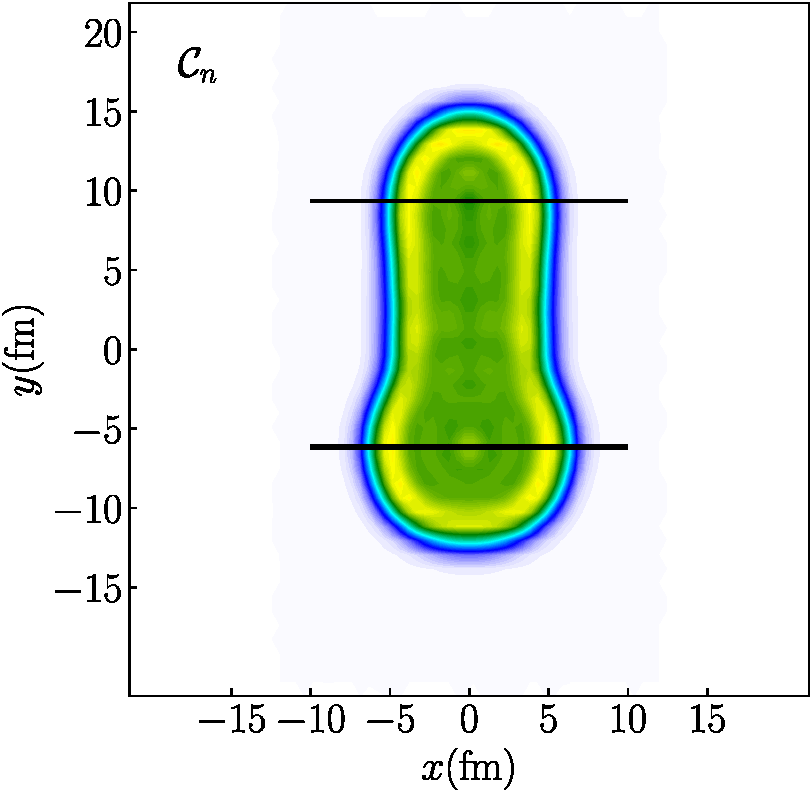
\includegraphics[width=0.35\linewidth]{TeX_files/rproc_254Pu_neutron} }}%
	\subfloat[$^{254}$Pu proton localization]{{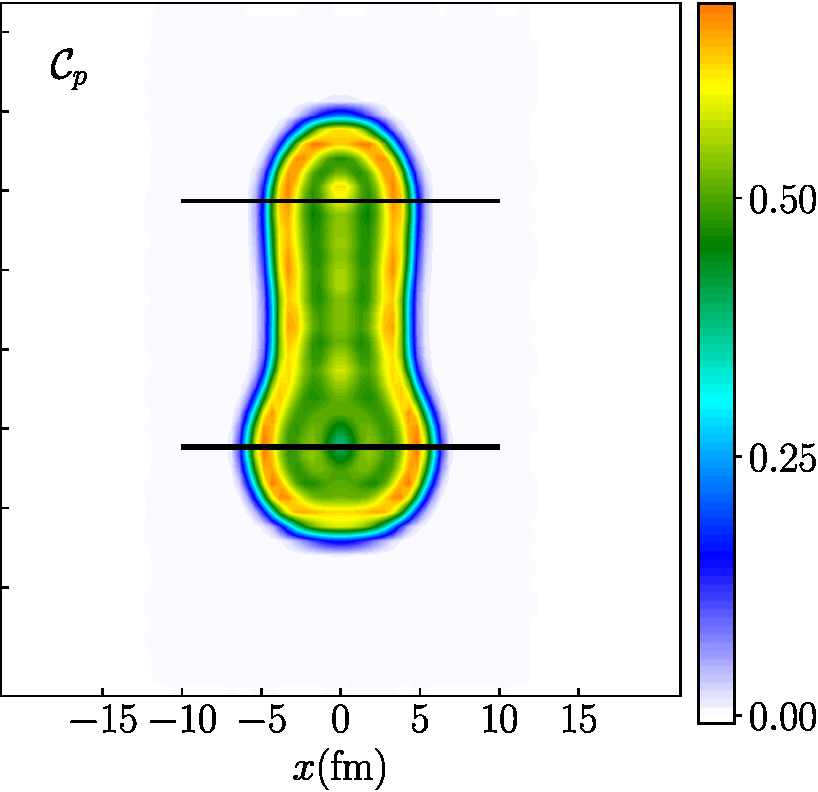
\includegraphics[width=0.355\linewidth]{TeX_files/rproc_254Pu_proton} }}%
%	\caption{Localization function for $^{254}$Pu with lines drawn to represent prefragment identification}%
%	\label{fig:254Pulocali}%
%\end{figure}
%
%
%\begin{figure}%
%	\centering
	\qquad
	\subfloat[$^{254}$Pu PES]{{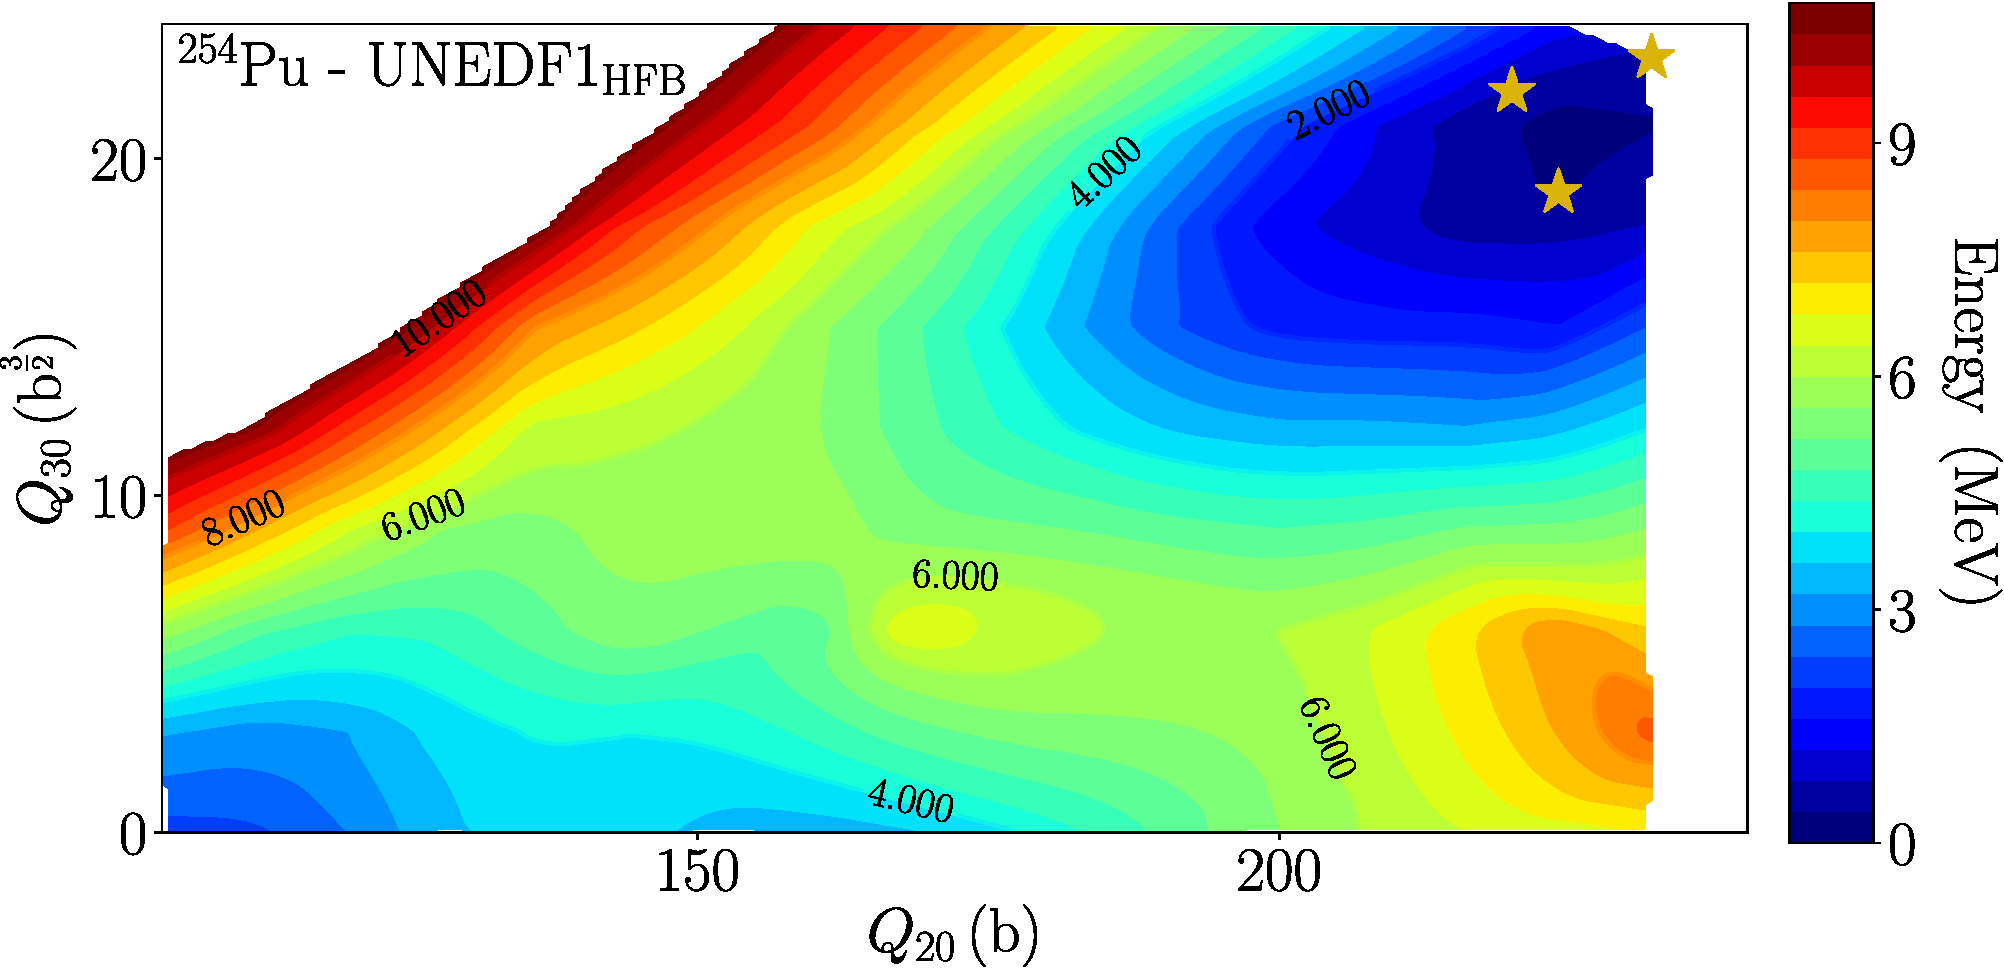
\includegraphics[width=0.8\linewidth]{TeX_files/rproc_254Pu-PES} }}%Normalized to gs energy, -1880.118539
	\qquad
	\subfloat[$^{254}$Pu yield]{{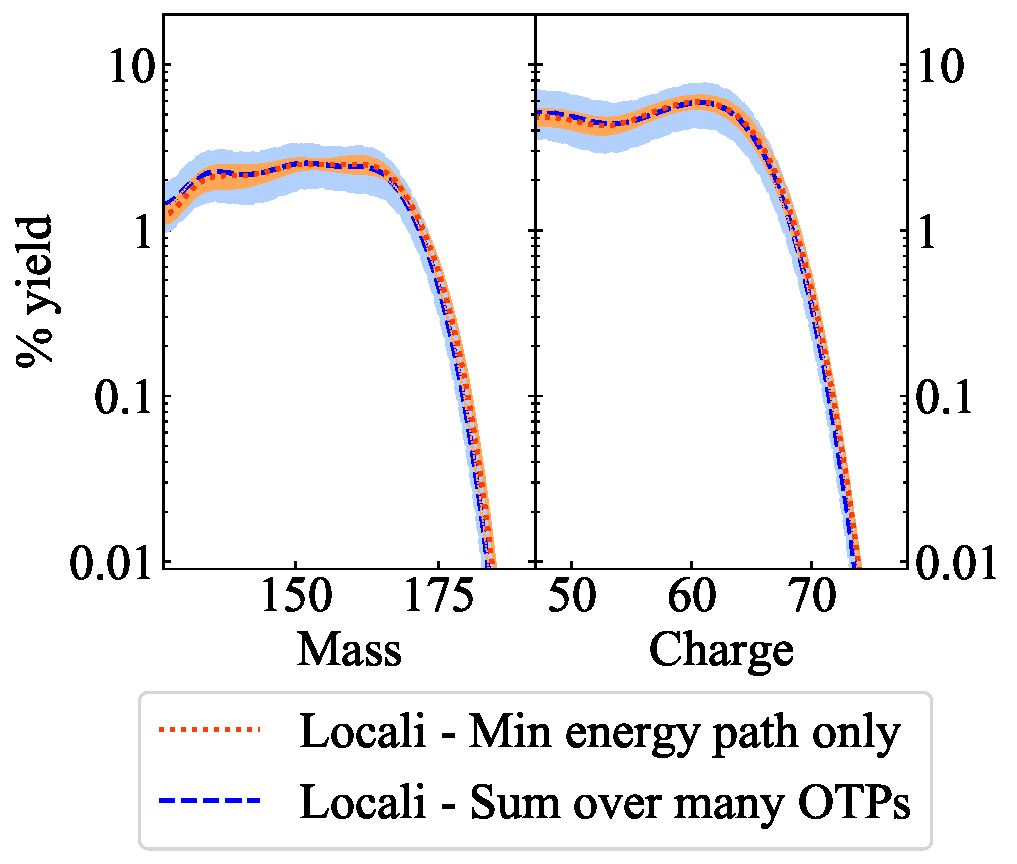
\includegraphics[width=0.5\linewidth]{TeX_files/rproc_254Pu-yield} }}%
	\caption{Localization function, PES, and yield distribution for the spontaneous fission of $^{254}$Pu. The stars in the PES indicate outer turning points which were used to compute the cumulative yields.}%
	\label{fig:254Pu-yield}%
\end{figure}

Looking first at the $^{254}$Pu localizations, we see a spherical heavy prefragment and a highly-elongated lighter prefragment connected by a thick neck. The spherical prefragment is well-localized, leading to a narrow uncertainty band in the overall yield. However, because of the large number of nucleons remaining in the neck, the statistical redistribution of neck particles produces a broad distribution of potential fragments. It would be interesting to see whether the peak will narrow and the lighter fragment will become better localized well-beyond the outer turning line, but that is beyond the scope of this project.

%Will you not also want/need to mention your work on 290Fm? This {\Cf} is not all that neutron rich, nor is it far from the region most-commonly studied. So perhaps you should say and do a bit more work on Fermium. Even just to say that triaxiality is not important here is something and not nothing. The reason you began to study this particular nucleus, though, is that based on Trevor Sprouse's r process network calculations (which utilized Peter Moller's fission calculations) and depending on the specifics of the astrophysical conditions, fission terminates the r process in a region of the N-Z plane. 290Fm falls into the range identified in one of these calculations (it would be good to cite it) and was selected by Trevor as one which may be particularly significant. However, looking back over my emails, it seems like this is not a robust finding. Other predictions (like the ones I have from Samuel and Marius Eichler) seem to perhaps indicate that I'd be better off looking in the region for which 280Fm is the northeast corner, perhaps.

Compared to $^{254}$Pu, the $^{290}$Fm nucleus is not as well-localized at the outer turning line, and a neck is only just starting to form in the protons. The neutron localization shows a ring- or disk-like of neutrons forming around the neck, which may lead to a large number of prompt neutrons being emitted. Because of this, the error bands associated with prefragment identification and the yields are much wider than for $^{254}$Pu. On the other hand, the overall distribution is much narrower, suggesting that symmetric fission will dominate for this nucleus. Yield contributions from mass-asymmetric outer turning points slightly broaden the neutron distribution, but they have almost no effect on the proton distribution, which remains peaked at $Z=54$.

\begin{figure}%
	\centering
	\subfloat[$^{290}$Fm neutron localization]{{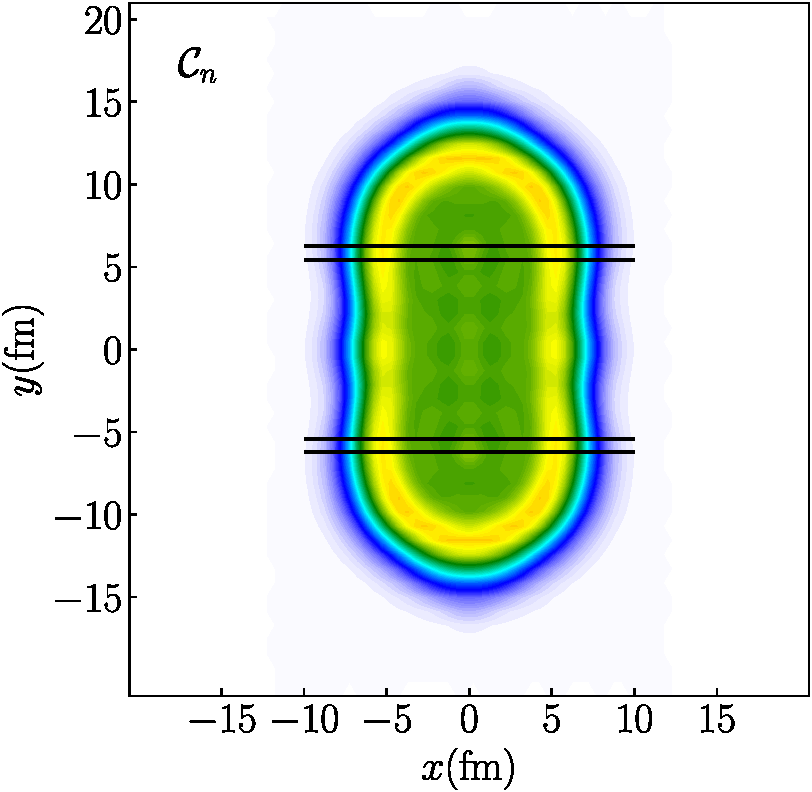
\includegraphics[width=0.35\linewidth]{TeX_files/rproc_290Fm_neutron} }}%
	\subfloat[$^{290}$Fm proton localization]{{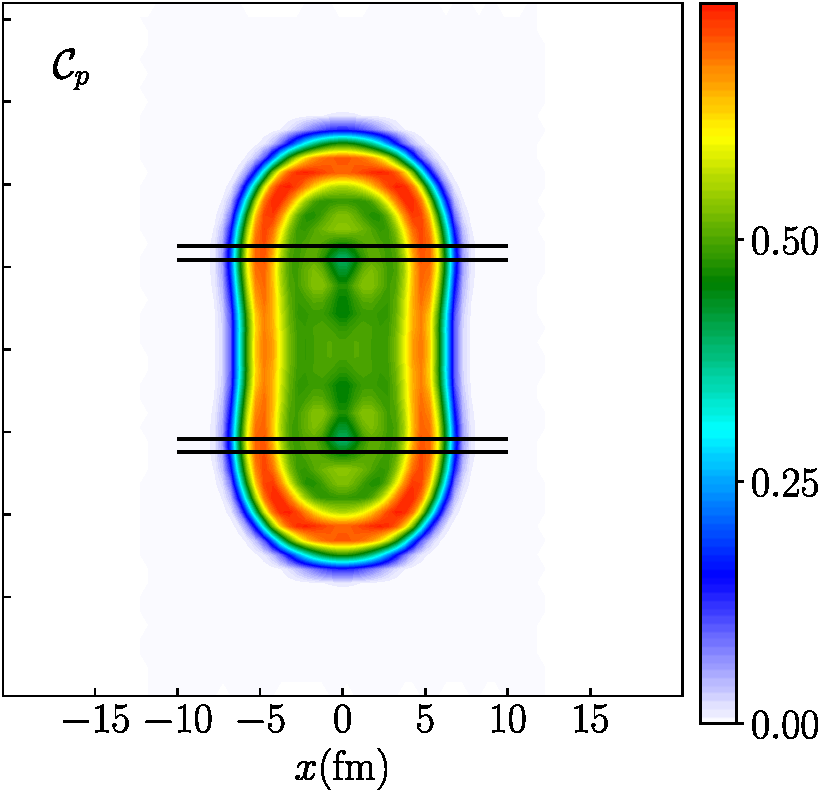
\includegraphics[width=0.355\linewidth]{TeX_files/rproc_290Fm_proton} }}%
%	\caption{Same as Figure~\ref{fig:254Pulocali} but for $^{290}$Fm.}%
%	\label{fig:290Fmlocali}%
%\end{figure}
%
%
%\begin{figure}%
%	\centering
	\qquad
	\subfloat[$^{290}$Fm PES]{{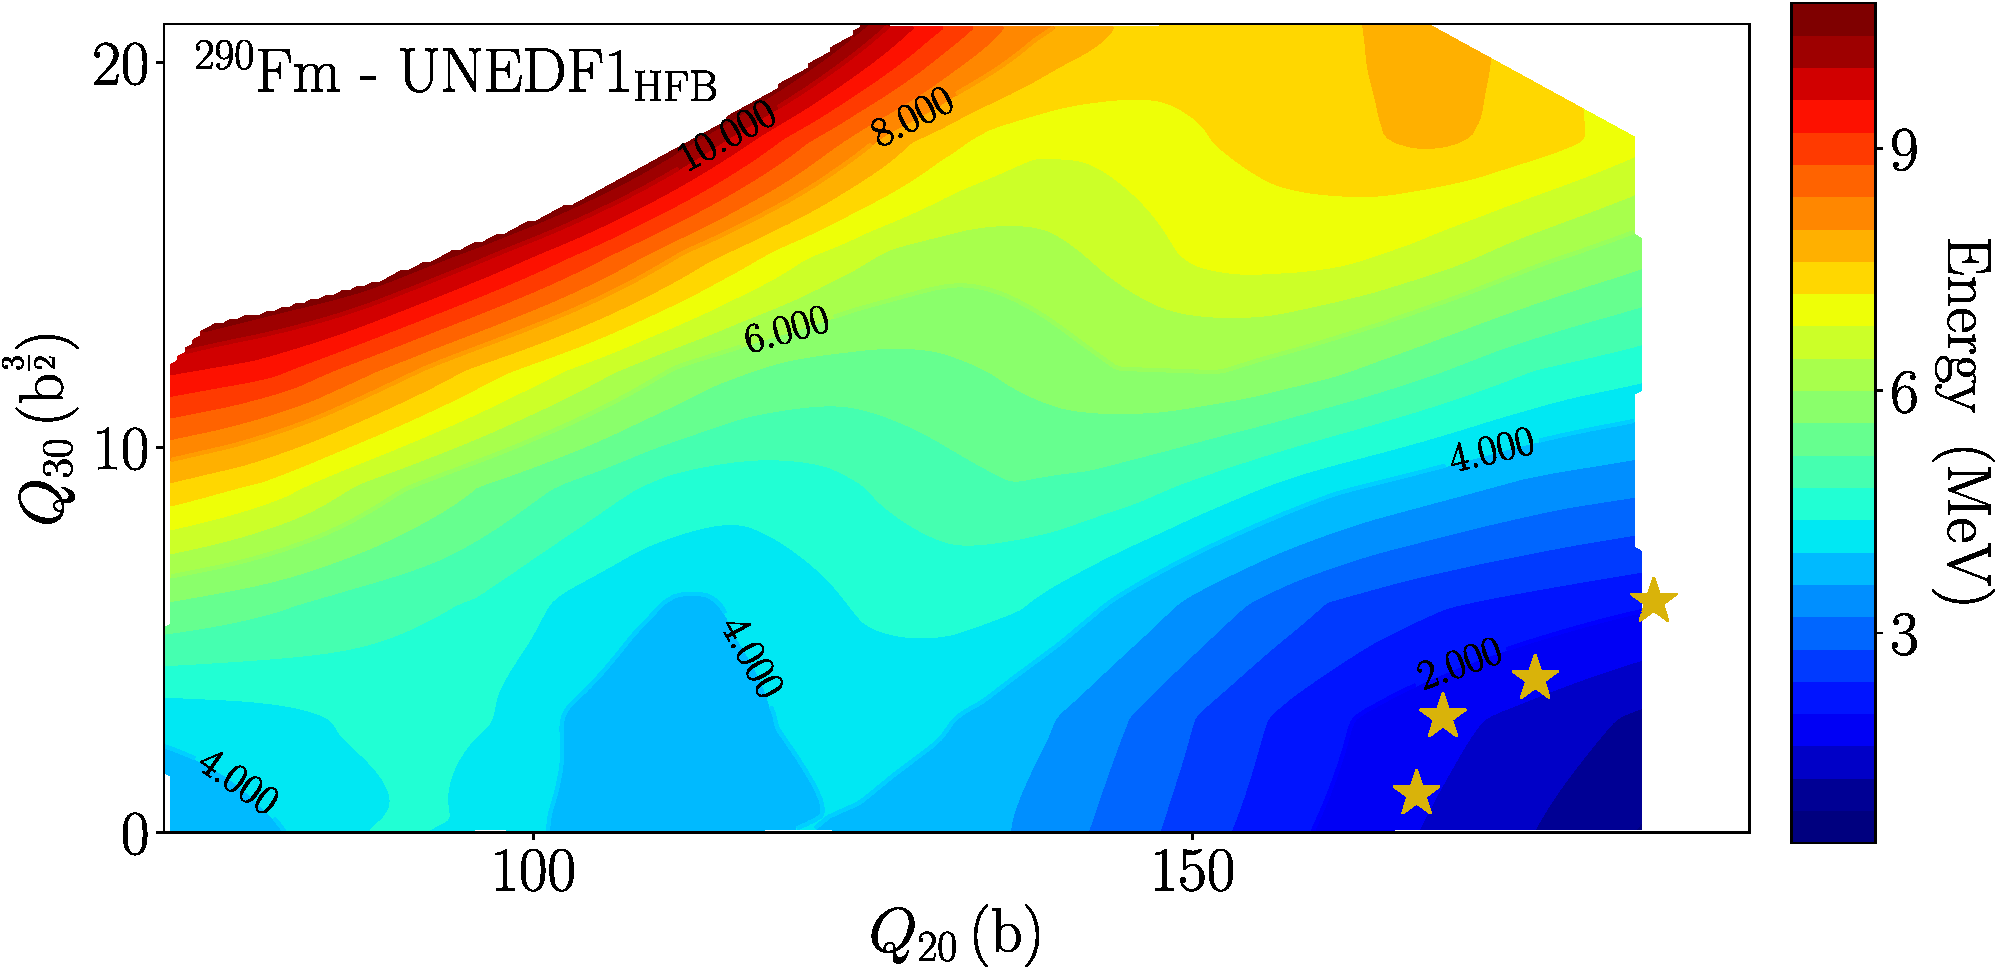
\includegraphics[width=0.8\linewidth]{TeX_files/rproc_290Fm-PES} }}%Normalized to gs energy, -2039.349002
	\qquad
	\subfloat[$^{290}$Fm yield]{{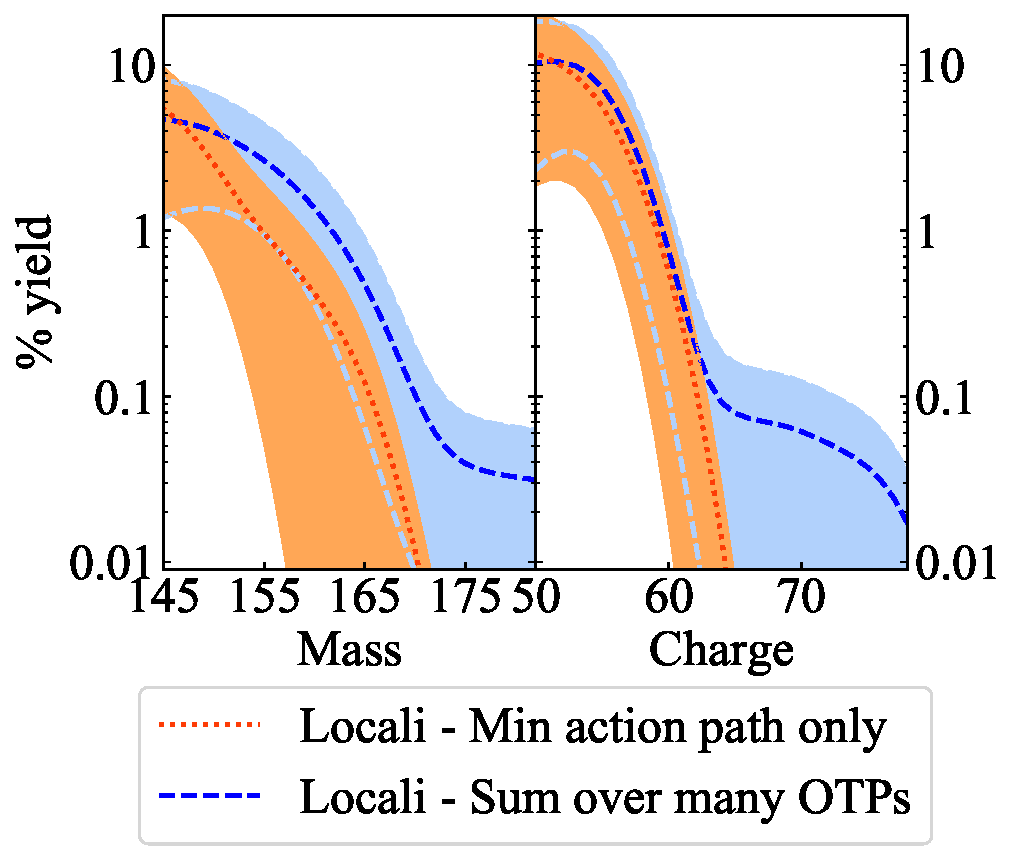
\includegraphics[width=0.5\linewidth]{TeX_files/rproc_290Fm-yield} }}%
	\caption{Similar to Figure~\ref{fig:254Pu-yield}, but for $^{290}$Fm.}%
	\label{fig:290Fm-yield}%
\end{figure}

\section{Future survey-level calculations for the r process}

Even with methods such as ours, which can reduce the computational burden, a survey-level calculation of fission fragment distributions across the nuclear chart, or even across the region relevant for r-process astrophysics, would be a major undertaking. A more efficient approach would be to isolate a small subset of fissioning nuclei which most affect the final abundance pattern, and make yield predictions for these first.

A modified sensitivity study was performed in~\cite{Vassh2019} in which, instead of assessing uncertainties, the goal was to isolate ``hot spots'' of nuclei that would have the greatest impact on the final r-process abundance pattern. Four different nuclear structure models were used to estimate these hot spots, with fission fragment yields provided by the phenomenological GEF model~\cite{Schmidt2016}. The neutron-induced fission hot spots are shown in Figure~\ref{fig:rprocimportant-fissions}, with the four different results superimposed on top of one another.

\begin{figure}
	\centering
	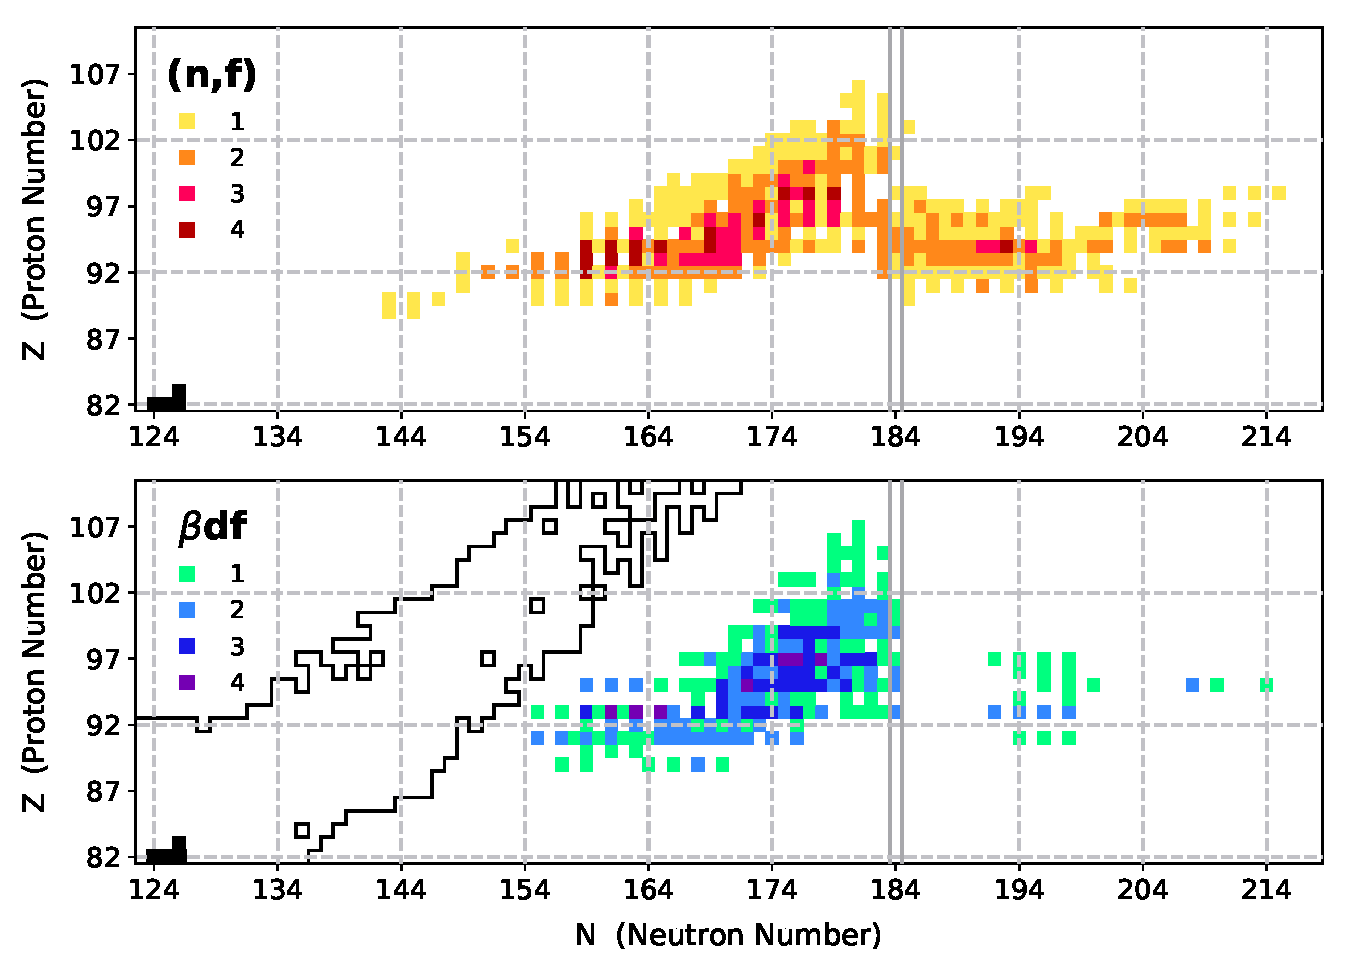
\includegraphics[width=0.7\linewidth]{TeX_files/rProc_important-fissions}
	\caption[Heatmap showing isotopes whose fission yields are especially relevant to the r process. This combines the results from four different nuclear structure models, and counts how many of the models found each isotope to have an integrated fission flow above a certain threshold.]{Heatmap showing isotopes whose fission yields are especially relevant to the r process. This combines the results from four different nuclear structure models, and counts how many of the models found each isotope to have an integrated fission flow above a certain threshold. Figure from~\cite{Vassh2019}.}
	\label{fig:rprocimportant-fissions}
\end{figure}

It should be noted that Figure~\ref{fig:rprocimportant-fissions} shows isotopes relevant specifically for their neutron-induced fission yields; however, the GEF yields on which the calculation was based do not show a strong dependence on excitation energy for many nuclei of interest. Therefore, as a first attempt, one might start simply by calculating the spontaneous fission yields for the isotopes indicated in Figure~\ref{fig:rprocimportant-fissions}. A proper treatment of neutron-induced fission using a finite temperature formalism is under development, but many challenges still remain (see Appendix~\ref{append:TD-ATDHFB} as well as ~\cite{Mcdonnell2014, Schunck2014, Schunck2015b}).

%\section{Kilonova and $^{254}$Cf}
%
%The environment in which the r process takes place is still an unresolved question. Core-collapse supernovae were a leading contender for years, but that hypothesis has recently fallen out of favor because the ejecta produced in such an event is not neutron-rich enough to host a strong r process \verb|\cite{???}|. Bolstered by theoretical calculations \verb|\cite{???}| and the neutron star merger event GW170817~\cite{Abbott2017,Abbott2017a}, neutron star mergers are now known to be a source of r-process nuclei; however it is not yet known if neutron star mergers can account for all of the observed r-process abundances~\cite{Pian2017,Kasen2017}. If it turns out that an additional r-process site is needed to explain stellar abundances, another possible location is a collapsar, which has not been observed but which matches the final abundances well in simulations~\cite{Nakamura2013,Siegel2018}. Regardless, the current results are far from conclusive, and stronger evidence is needed.
%
%A neutron star merger produces a bright burst of electromagnetic radiation called a kilonova, which is caused by residual radioactivity as neutron-rich material produced in the merger decays toward stability. This material produces an observable light curve, which is one way to characterize the kilonova. A kilonova was actually observed in the GW170817 event, providing confirmation of theoretical predictions along with a great deal of useful experimental data~\cite{drout2017}. The light curve will be dominated by radiation from alpha and beta decay events at early times, but if nuclei with spontaneous fission half-lives on the order of several days are produced in sufficient quantities, these would have a major impact on late-time heating in the kilonova, which would in turn affect the light curve. Thus, the shape of the light curve may indicate whether or not heavy, short-lived actinides were produced in a neutron star merger, and in turn help us answer the question of where the r process takes place.
%
%The question remains whether such nuclei exist. Limiting ourselves to isotopes that have been experimentally measured, there are several which primarily undergo spontaneous fission and which may be produced in sufficient quantities during the r process to impact the light curve: several isotopes each of californium and fermium, plus $^{260}$Md. However, most of the fermium and californium isotopes are too short-lived, and the population of $^{260}$Md during the r process is highly model-dependent, leaving {\Cf} ($\tau_\frac{1}{2} = 60.5$days~\cite{NuDat}) as the most-likely candidate~\cite{Zhu2018}.% Sam has a few more references to site this in his network calulation -> abundances paper
%
%The effect of {\Cf} on kilonova heating and the light curve depends on the energy released during fission, which in turn depends on the fragment yield it produces. Mass and kinetic energy distributions of {\Cf} were actually measured in~\cite{Brandt1963}, but for some reason, Zhu considers that measurement ``sparse'' and they do some dressing up of it in their paper~\cite{Zhu2018}. We decide to compute it microscopically using our Langevin approach, just to see what useful information we can add.



%Kilonova - the bright burst of gamma rays and other radiation that accompanies a compact object merger, presumably created mainly from the radioactive decay of unstable r-process nuclei (mainly via alpha and beta decay, but not fission - according to \verb|https://www.nndc.bnl.gov/fire/documents/FIRE_DOE_Yonglin.pdf|; see also the paper~\cite{Zhu2018})
%
%Light curves - show the magnitude/intensity of light/EM radiation as a function of time. For example, the light curve from the sun on the earth will be roughly sinusoidal; from an eclipse, you'll have a roughly straight line, then a dip, then a return to the original straight line; a pulsar will also be something regular and periodic. Each type of nova/supernova/kilonova/etc. has its own characteristic light curve, with an initial peak of varying sharpness, and then a gradual decay (though how gradual depends on the characteristics of the event).
%
%Heating - Is exactly what it sounds like. When a nucleus decays, it loses energy. Some of that energy escapes in the form of neutrinos or photons, while other energy is absorbed elsewhere in the medium. A related concept is opacity. Heavier nuclei with a large level density tend to be more opaque because they can more readily absorb photons than smaller, less opaque nuclei. And the process by which all of this energy exchange takes place is called thermalization.


